\documentclass[aspectratio=169,10pt]{beamer}

\usepackage[T1]{fontenc}
\usepackage[utf8]{inputenc}
\usepackage{lmodern}
\usepackage{microtype}
\usepackage{amssymb}
\usepackage{tikz}
\usetikzlibrary{arrows.meta,positioning,calc}
\usepackage{ragged2e}
\usepackage{array}

\renewcommand{\familydefault}{\sfdefault}
\setbeamertemplate{navigation symbols}{}
\setbeamersize{text margin left=0.72cm,text margin right=0.72cm}

\definecolor{Paper}{HTML}{F5F6F2}
\definecolor{White}{HTML}{FFFFFF}
\definecolor{Ink}{HTML}{151A17}
\definecolor{Muted}{HTML}{626B65}
\definecolor{Line}{HTML}{DCE1DA}
\definecolor{Acid}{HTML}{D7FB63}
\definecolor{Orange}{HTML}{FF7557}
\definecolor{Green}{HTML}{174B3A}
\definecolor{Soft}{HTML}{E9EEE4}
\definecolor{Deep}{HTML}{202923}

\setbeamercolor{normal text}{fg=Ink,bg=Paper}
\setbeamercolor{structure}{fg=Green}
\setbeamercolor{frametitle}{fg=Ink,bg=Paper}
\setbeamercolor{footline}{fg=Muted,bg=Paper}
\setbeamerfont{frametitle}{family=\sffamily,series=\bfseries,size=\Large}
\setbeamertemplate{itemize item}{\color{Orange}\raisebox{0.15ex}{\tiny$\blacksquare$}}
\setbeamertemplate{itemize subitem}{\color{Green}\raisebox{0.15ex}{\tiny$\blacktriangleright$}}

\setbeamertemplate{footline}{%
  \leavevmode%
  \hbox{%
    \begin{beamercolorbox}[wd=.72\paperwidth,ht=2.7ex,dp=1.2ex,leftskip=.72cm]{footline}%
      \textsf{\bfseries proof}\hspace{.5em}\textcolor{Line}{|}\hspace{.5em}Investor overview
    \end{beamercolorbox}%
    \begin{beamercolorbox}[wd=.28\paperwidth,ht=2.7ex,dp=1.2ex,rightskip=.72cm plus1fil]{footline}%
      \hfill\insertframenumber\,/\,10
    \end{beamercolorbox}%
  }%
}

\newcommand{\kicker}[1]{\textcolor{Green}{\fontsize{7.5}{9}\selectfont\ttfamily\MakeUppercase{#1}}}
\newcommand{\titleline}[2]{%
  {\kicker{#1}}\\[-1pt]
  {\fontsize{23}{26}\selectfont\bfseries #2}\\[3pt]
}
\newcommand{\smallrule}{\textcolor{Line}{\rule{\linewidth}{.6pt}}}
\newcommand{\decktag}[1]{\tikz[baseline=(n.base)]\node[draw=Line,fill=White,inner xsep=5pt,inner ysep=2pt,font=\fontsize{7}{8}\selectfont\ttfamily,text=Muted] (n) {#1};}
\newcommand{\bigstat}[2]{\textcolor{Green}{\fontsize{19}{21}\selectfont\bfseries #1}\\[-1pt]{\fontsize{8}{10}\selectfont\color{Muted}#2}}
\newcommand{\flowtitle}{\fontsize{12}{14}\selectfont\bfseries\color{Ink}}
\newcommand{\flowcopy}{\fontsize{8}{11}\selectfont\color{Muted}}

\begin{document}

% 1. Opening
\begin{frame}[plain]
  \begin{tikzpicture}[remember picture,overlay]
    \fill[Paper] (current page.south west) rectangle (current page.north east);
    \fill[Deep] ([xshift=-5.55cm]current page.north east) rectangle (current page.south east);
    \fill[Acid] ([xshift=-5.55cm,yshift=-.45cm]current page.north east) rectangle ([xshift=-5.25cm,yshift=-.75cm]current page.north east);
    \foreach \x in {0,...,8} \foreach \y in {0,...,5}
      \fill[White,opacity=.12] ([xshift=-4.95cm+\x*.48cm,yshift=-1.0cm-\y*.48cm]current page.north east) circle (0.7pt);
    \draw[Green,line width=1pt] ([xshift=.72cm,yshift=-.78cm]current page.north west) -- ++(.29cm,0) -- ++(0,-.29cm);
    \node[anchor=north west,text=White,font=\fontsize{8}{10}\selectfont\ttfamily] at ([xshift=-5.02cm,yshift=-.72cm]current page.north east) {PROOF / WORK RECORD};
    \node[anchor=south east,text=White,font=\fontsize{8}{10}\selectfont\ttfamily] at ([xshift=-.55cm,yshift=.4cm]current page.south east) {PRODUCT PREVIEW / DEMO DATA};
    \node[anchor=north west,draw=Line,fill=White,minimum width=4.15cm,minimum height=1.25cm,align=left,inner sep=10pt] (profile) at ([xshift=-4.95cm,yshift=-1.65cm]current page.north east) {\textcolor{Muted}{\fontsize{7}{9}\selectfont PROFESSIONAL PROFILE}\\[-1pt]\textbf{Maya Chen}\\[-2pt]{\color{Muted}\fontsize{8}{10}\selectfont AI systems engineer}};
    \node[anchor=north west,draw=Acid,fill=Deep,text=White,minimum width=4.15cm,minimum height=2.0cm,align=left,inner sep=10pt] (evidence) at ([xshift=-4.95cm,yshift=-3.22cm]current page.north east) {\textcolor{Acid}{\fontsize{7}{9}\selectfont SESSION EVIDENCE}\\[3pt]\textbf{Reliability review}\\[-1pt]{\color{White!72}\fontsize{8}{10}\selectfont Decisions, corrections, shared work, and a report.}\\[7pt]\textcolor{Acid}{\fontsize{7}{9}\selectfont ILLUSTRATIVE DEMO DATA}};
    \draw[-{Stealth[length=2mm]},color=Acid,line width=.8pt] (profile.south west) ++(.35cm,0) -- ++(0,-.27cm);
  \end{tikzpicture}
  \vspace*{1.0cm}
  \hspace*{.72cm}\begin{minipage}[t][5.3cm][t]{7.25cm}
    \kicker{Professional identity, backed by work}\\[.4cm]
    {\fontsize{31}{34}\selectfont\bfseries Make professional\\reputation\\\textcolor{Green}{inspectable.}}\\[.45cm]
    {\fontsize{11}{15}\selectfont\color{Muted}A professional network where collaboration, completed work, and performance history become part of the profile.}\\[.65cm]
    \decktag{INVESTOR OVERVIEW}\hspace{.2cm}\decktag{OCTOBER 2026}
  \end{minipage}
\end{frame}

% 2. Problem
\begin{frame}
  \titleline{01 / THE PROBLEM}{Hiring sees the profile. It misses the work.}
  \vspace{.35cm}
  \begin{columns}[T,onlytextwidth]
    \column{.31\textwidth}
      {\color{Orange}\fontsize{10}{12}\selectfont\ttfamily 01}\\[.35cm]
      {\fontsize{16}{19}\selectfont\bfseries Claims are easy to polish}\\[.18cm]
      {\fontsize{9.5}{13}\selectfont\color{Muted}Resumes, portfolios, and credentials describe a person, but rarely show how their work unfolded.}
    \column{.035\textwidth}\centering\textcolor{Line}{\rule{.5pt}{3.45cm}}
    \column{.31\textwidth}
      {\color{Orange}\fontsize{10}{12}\selectfont\ttfamily 02}\\[.35cm]
      {\fontsize{16}{19}\selectfont\bfseries Interviews are snapshots}\\[.18cm]
      {\fontsize{9.5}{13}\selectfont\color{Muted}Short conversations compress reasoning, collaboration, and judgment into a narrow window.}
    \column{.035\textwidth}\centering\textcolor{Line}{\rule{.5pt}{3.45cm}}
    \column{.31\textwidth}
      {\color{Orange}\fontsize{10}{12}\selectfont\ttfamily 03}\\[.35cm]
      {\fontsize{16}{19}\selectfont\bfseries Context gets discarded}\\[.18cm]
      {\fontsize{9.5}{13}\selectfont\color{Muted}Most hiring records capture the answer, not the decisions, revisions, and teamwork behind it.}
  \end{columns}
  \vfill
  \colorbox{Ink}{\parbox{\dimexpr\linewidth-2\fboxsep}{\vspace{.18cm}\hspace{.18cm}\textcolor{Acid}{\bfseries The gap}\hspace{.35cm}\textcolor{White}{A professional record should carry more than self-reported claims.}\vspace{.18cm}}}
\end{frame}

% 3. Solution
\begin{frame}
  \titleline{02 / THE PRODUCT}{Proof connects the work to the professional record.}
  \vspace{.25cm}
  \begin{center}
  \begin{tikzpicture}[
    node distance=4mm,
    flowbox/.style={draw=Line,fill=White,minimum width=3.12cm,minimum height=2.45cm,align=left,inner sep=9pt,anchor=north west},
    flowcopy/.style={font=\fontsize{8}{11}\selectfont,text=Muted}
  ]
    \node[flowbox] (a) at (0,0) {\textcolor{Green}{\fontsize{8}{10}\selectfont\ttfamily 01 / ROOM}\\[.25cm]{\flowtitle Shared work}\\[.15cm]{\flowcopy People solve a real problem together in a structured room.}};
    \node[flowbox,right=of a] (b) {\textcolor{Green}{\fontsize{8}{10}\selectfont\ttfamily 02 / TRACE}\\[.25cm]{\flowtitle Session events}\\[.15cm]{\flowcopy The system records activity and outcomes as session evidence.}};
    \node[flowbox,right=of b] (c) {\textcolor{Green}{\fontsize{8}{10}\selectfont\ttfamily 03 / REPORT}\\[.25cm]{\flowtitle Analysis}\\[.15cm]{\flowcopy A report organizes observations, strengths, and development areas.}};
    \node[flowbox,right=of c] (d) {\textcolor{Green}{\fontsize{8}{10}\selectfont\ttfamily 04 / PROFILE}\\[.25cm]{\flowtitle Work history}\\[.15cm]{\flowcopy The professional profile brings evidence together over time.}};
    \draw[-{Stealth[length=2mm]},line width=1pt,color=Orange] (a.east) -- (b.west);
    \draw[-{Stealth[length=2mm]},line width=1pt,color=Orange] (b.east) -- (c.west);
    \draw[-{Stealth[length=2mm]},line width=1pt,color=Orange] (c.east) -- (d.west);
  \end{tikzpicture}
  \end{center}
  \vspace{.45cm}
  \begin{columns}[T,onlytextwidth]
    \column{.49\textwidth}{\fontsize{9}{12}\selectfont\color{Muted}A session can be a coding room, design review, business case, research discussion, or structured interview.}
    \column{.49\textwidth}{\fontsize{9}{12}\selectfont\color{Muted}The same product connects professional profiles, a network, and hiring-team workflows.}
  \end{columns}
\end{frame}

% 4. Product surface
\begin{frame}
  \titleline{03 / PRODUCT SURFACE}{A professional network built around demonstrated work.}
  \vspace{.15cm}
  \begin{columns}[T,onlytextwidth]
    \column{.47\textwidth}
      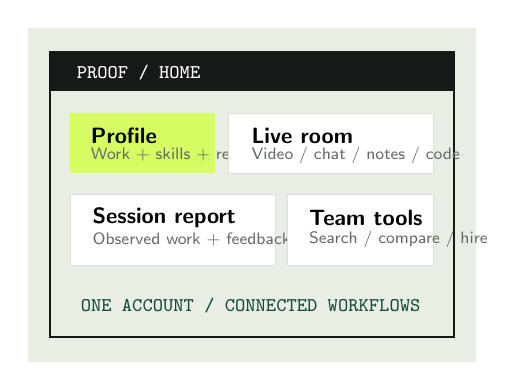
\begin{tikzpicture}[x=1cm,y=1cm]
        \fill[Soft] (0,0) rectangle (5.7,4.25);
        \draw[Ink,line width=.7pt] (.28,.32) rectangle (5.42,3.94);
        \fill[Ink] (.28,3.44) rectangle (5.42,3.94);
        \node[anchor=west,text=White,font=\fontsize{7}{9}\selectfont\ttfamily] at (.5,3.68) {PROOF / HOME};
        \fill[Acid] (.54,2.4) rectangle (2.38,3.16);
        \node[anchor=west,font=\fontsize{8}{10}\selectfont\bfseries] at (.68,2.88) {Profile};
        \node[anchor=west,text=Muted,font=\fontsize{6.5}{8}\selectfont] at (.68,2.63) {Work + skills + reports};
        \fill[White] (2.55,2.4) rectangle (5.15,3.16);
        \draw[Line] (2.55,2.4) rectangle (5.15,3.16);
        \node[anchor=west,font=\fontsize{8}{10}\selectfont\bfseries] at (2.72,2.88) {Live room};
        \node[anchor=west,text=Muted,font=\fontsize{6.5}{8}\selectfont] at (2.72,2.63) {Video / chat / notes / code};
        \fill[White] (.54,1.23) rectangle (3.15,2.13);
        \draw[Line] (.54,1.23) rectangle (3.15,2.13);
        \node[anchor=west,font=\fontsize{8}{10}\selectfont\bfseries] at (.7,1.83) {Session report};
        \node[anchor=west,text=Muted,font=\fontsize{6.5}{8}\selectfont] at (.7,1.56) {Observed work + feedback};
        \fill[White] (3.3,1.23) rectangle (5.15,2.13);
        \draw[Line] (3.3,1.23) rectangle (5.15,2.13);
        \node[anchor=west,font=\fontsize{8}{10}\selectfont\bfseries] at (3.45,1.83) {Team tools};
        \node[anchor=west,text=Muted,font=\fontsize{6.5}{8}\selectfont] at (3.45,1.56) {Search / compare / hire};
        \node[anchor=west,text=Green,font=\fontsize{7}{9}\selectfont\ttfamily] at (.55,.72) {ONE ACCOUNT / CONNECTED WORKFLOWS};
      \end{tikzpicture}
    \column{.49\textwidth}
      \vspace{.12cm}
      \textbf{For professionals}\\[-1pt]{\fontsize{8.5}{11}\selectfont\color{Muted}Build a profile with experience, projects, credentials, skills, and completed session reports.}\\[.32cm]
      \textbf{For collaborators}\\[-1pt]{\fontsize{8.5}{11}\selectfont\color{Muted}Work in rooms with video, chat, notes, whiteboards, and code.}\\[.32cm]
      \textbf{For hiring teams}\\[-1pt]{\fontsize{8.5}{11}\selectfont\color{Muted}Search profiles, compare candidates, manage jobs and applications, and invite people to structured sessions.}\\[.32cm]
      \decktag{Illustrative product map}
  \end{columns}
\end{frame}

% 5. Room experience
\begin{frame}
  \titleline{04 / THE ROOM}{A shared workspace for work that is hard to fake with a form.}
  \vspace{.25cm}
  \begin{columns}[T,onlytextwidth]
    \column{.23\textwidth}\bigstat{01}{Set the context}\\[.25cm]{\fontsize{8}{11}\selectfont\color{Muted}Choose a room format for the work: engineering, data, design, strategy, research, or an interview.}
    \column{.025\textwidth}\centering\textcolor{Orange}{\Large $\rightarrow$}
    \column{.23\textwidth}\bigstat{02}{Work together}\\[.25cm]{\fontsize{8}{11}\selectfont\color{Muted}Participants collaborate with the tools the session needs, not a one-size-fits-all quiz.}
    \column{.025\textwidth}\centering\textcolor{Orange}{\Large $\rightarrow$}
    \column{.23\textwidth}\bigstat{03}{Review the record}\\[.25cm]{\fontsize{8}{11}\selectfont\color{Muted}Session activity and outcomes feed into a report that can be reviewed in context.}
    \column{.025\textwidth}\centering\textcolor{Orange}{\Large $\rightarrow$}
    \column{.23\textwidth}\bigstat{04}{Keep building}\\[.25cm]{\fontsize{8}{11}\selectfont\color{Muted}Reports and professional history accumulate in a profile over time.}
  \end{columns}
  \vfill
  \smallrule\\[.2cm]
  \decktag{VIDEO}\hspace{.1cm}\decktag{CHAT}\hspace{.1cm}\decktag{NOTES}\hspace{.1cm}\decktag{WHITEBOARD}\hspace{.1cm}\decktag{CODE}\hspace{.3cm}{\fontsize{8}{10}\selectfont\color{Muted}Tools vary by room format.}
\end{frame}

% 6. Evidence
\begin{frame}
  \titleline{05 / EVIDENCE}{A report adds context. It is a signal, not a verdict.}
  \vspace{.15cm}
  \begin{columns}[T,onlytextwidth]
    \column{.51\textwidth}
      {\fontsize{10}{13}\selectfont\bfseries What the system does}\\[.3cm]
      \begin{itemize}
        \item {\fontsize{8.5}{11}\selectfont\color{Muted}Stores ordered room events and session outcomes.}
        \item {\fontsize{8.5}{11}\selectfont\color{Muted}Analyzes evidence after a room is completed.}
        \item {\fontsize{8.5}{11}\selectfont\color{Muted}Produces reports with strengths, development areas, suggestions, and performance metrics.}
        \item {\fontsize{8.5}{11}\selectfont\color{Muted}Supports deterministic scoring when optional AI analysis is unavailable.}
      \end{itemize}
      \vspace{.1cm}
      {\fontsize{8}{11}\selectfont\color{Muted}Evidence should be reviewed with the task, participants, and context in view. A score does not guarantee job performance.}
    \column{.045\textwidth}
    \column{.425\textwidth}
      \begin{tikzpicture}
        \node[anchor=north west,fill=Ink,text=White,minimum width=5.55cm,minimum height=4.22cm,inner sep=12pt,align=left] at (0,0) {\textcolor{Acid}{\fontsize{7}{9}\selectfont\ttfamily SESSION REPORT / EXAMPLE}\\[.18cm]
          {\fontsize{14}{17}\selectfont\bfseries Reliability review}\\[.08cm]
          {\fontsize{8}{10}\selectfont\color{White!70}Structured session / report view}\\[.22cm]
          \textcolor{White!36}{\rule{4.9cm}{.4pt}}\\[.19cm]
          {\fontsize{7}{9}\selectfont\color{Acid}\ttfamily OBSERVED STRENGTH}\\[-1pt]
          {\fontsize{8}{10}\selectfontReframed the problem around observability.}\\[.17cm]
          {\fontsize{7}{9}\selectfont\color{Acid}\ttfamily REVIEW CONTEXT}\\[-1pt]
          {\fontsize{8}{10}\selectfontAssumptions, revisions, and shared decisions.}\\[.17cm]
          {\fontsize{7}{9}\selectfont\color{Acid}\ttfamily NEXT QUESTION}\\[-1pt]
          {\fontsize{8}{10}\selectfontWhich trade-off changed the final recommendation?}\\[.22cm]
          {\fontsize{6.5}{8}\selectfont\color{White!60}ILLUSTRATIVE REPORT CONTENT}}
      \end{tikzpicture}
  \end{columns}
\end{frame}

% 7. Architecture
\begin{frame}
  \titleline{06 / TECHNOLOGY}{A full-stack product, with a clear production boundary.}
  \vspace{.12cm}
  \begin{center}
    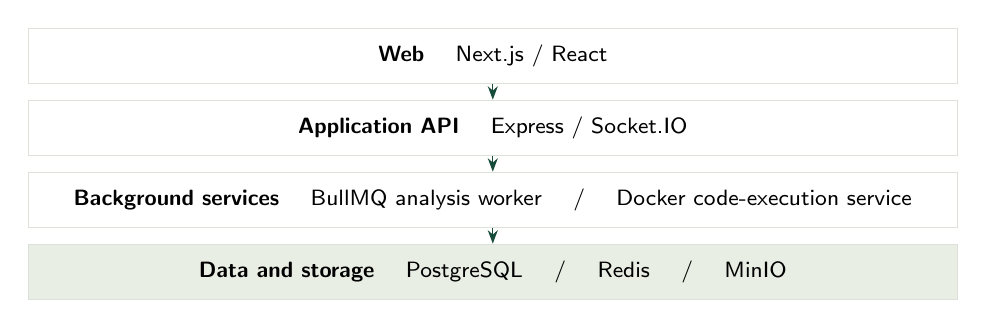
\begin{tikzpicture}[
      layer/.style={draw=Line,fill=White,minimum height=.7cm,align=center,font=\fontsize{8}{10}\selectfont},
      node distance=2mm
    ]
      \node[layer,minimum width=11.8cm] (web) {\textbf{Web} \quad Next.js / React};
      \node[layer,minimum width=11.8cm,below=of web] (api) {\textbf{Application API} \quad Express / Socket.IO};
      \node[layer,minimum width=11.8cm,below=of api] (services) {\textbf{Background services} \quad BullMQ analysis worker \quad / \quad Docker code-execution service};
      \node[layer,minimum width=11.8cm,below=of services,fill=Soft] (data) {\textbf{Data and storage} \quad PostgreSQL \quad / \quad Redis \quad / \quad MinIO};
      \draw[-{Stealth[length=1.7mm]},color=Green] (web) -- (api);
      \draw[-{Stealth[length=1.7mm]},color=Green] (api) -- (services);
      \draw[-{Stealth[length=1.7mm]},color=Green] (services) -- (data);
    \end{tikzpicture}
  \end{center}
  \vspace{.24cm}
  \colorbox{Ink}{\parbox{\dimexpr\linewidth-2\fboxsep}{\vspace{.13cm}\hspace{.16cm}{\color{Acid}\bfseries Current boundary}\hspace{.3cm}{\color{White}\fontsize{8}{10}\selectfont The all-in-one source release runs locally. Public scale still needs managed infrastructure, production media routing, hardened execution, billing and email, security review, and load testing.}\vspace{.13cm}}}
\end{frame}

% 8. Business model
\begin{frame}
  \titleline{07 / BUSINESS MODEL}{Start with the team workflow. Test the network effect.}
  \vspace{.25cm}
  \begin{columns}[T,onlytextwidth]
    \column{.47\textwidth}
      \colorbox{Acid}{\parbox{\dimexpr\linewidth-2\fboxsep}{\vspace{.18cm}\hspace{.15cm}{\fontsize{7}{9}\selectfont\ttfamily INITIAL BUYER HYPOTHESIS}\vspace{.1cm}\\\hspace{.15cm}{\fontsize{16}{19}\selectfont\bfseries Hiring teams}\vspace{.18cm}}}\\[.35cm]
      {\fontsize{9}{12}\selectfont\bfseries Potential paid workflows}\\[.15cm]
      {\fontsize{8.5}{11}\selectfont\color{Muted}Company workspaces, candidate discovery and comparison, job workflows, and structured assessments.}\\[.25cm]
      {\fontsize{8}{11}\selectfont\color{Muted}A team subscription is a direction to validate; no pricing or willingness-to-pay evidence is claimed here.}
    \column{.06\textwidth}
    \column{.47\textwidth}
      {\fontsize{9}{12}\selectfont\bfseries The participation loop}\\[.15cm]
      {\fontsize{8.5}{11}\selectfont\color{Muted}Professionals build a useful work record. Teams review richer context. Sessions create more evidence.}\\[.4cm]
      \smallrule\\[.25cm]
      {\fontsize{9}{12}\selectfont\bfseries Go-to-market to test}\\[.15cm]
      {\fontsize{8.5}{11}\selectfont\color{Muted}Recruit a small set of employers and recruiting teams as design partners. Test one repeated evaluation workflow before widening the market.}\\[.25cm]
      \decktag{PLG IS A HYPOTHESIS, NOT A METRIC}
  \end{columns}
\end{frame}

% 9. Stage
\begin{frame}
  \titleline{08 / CURRENT STAGE}{The product exists. Commercial evidence is next.}
  \vspace{.25cm}
  \begin{columns}[T,onlytextwidth]
    \column{.31\textwidth}
      \textcolor{Green}{\fontsize{8}{10}\selectfont\ttfamily BUILT}\\[.22cm]
      {\fontsize{14}{17}\selectfont\bfseries End-to-end product surface}\\[.15cm]
      {\fontsize{8.5}{11}\selectfont\color{Muted}Profiles, rooms, session reports, network features, jobs, company tools, and an investor demo dataset are present in the source release.}
    \column{.035\textwidth}\centering\textcolor{Line}{\rule{.5pt}{3.5cm}}
    \column{.31\textwidth}
      \textcolor{Orange}{\fontsize{8}{10}\selectfont\ttfamily TO VALIDATE}\\[.22cm]
      {\fontsize{14}{17}\selectfont\bfseries Repeat use and buyer value}\\[.15cm]
      {\fontsize{8.5}{11}\selectfont\color{Muted}Whether teams return, whether evidence changes decisions, and whether a buyer will pay for the workflow.}
    \column{.035\textwidth}\centering\textcolor{Line}{\rule{.5pt}{3.5cm}}
    \column{.31\textwidth}
      \textcolor{Orange}{\fontsize{8}{10}\selectfont\ttfamily TO HARDEN}\\[.22cm]
      {\fontsize{14}{17}\selectfont\bfseries Public-service readiness}\\[.15cm]
      {\fontsize{8.5}{11}\selectfont\color{Muted}Security, media, code isolation, operating costs, and deployment need production validation.}
  \end{columns}
  \vfill
  \colorbox{Soft}{\parbox{\dimexpr\linewidth-2\fboxsep}{\vspace{.16cm}\hspace{.16cm}{\bfseries Investor transparency}\hspace{.3cm}{\fontsize{8}{10}\selectfont No independently verified customer, revenue, pilot, or growth metrics are included in the materials reviewed.}\vspace{.16cm}}}
\end{frame}

% 10. Ask
\begin{frame}[plain]
  \begin{tikzpicture}[remember picture,overlay]
    \fill[Ink] (current page.south west) rectangle (current page.north east);
    \fill[Acid] (current page.north east) rectangle ([xshift=-.28cm,yshift=-.28cm]current page.north east);
    \foreach \x in {0,...,10} \foreach \y in {0,...,5}
      \fill[White,opacity=.08] ([xshift=.7cm+\x*.48cm,yshift=-.7cm-\y*.48cm]current page.north west) circle (.65pt);
  \end{tikzpicture}
  \vspace*{.8cm}
  \hspace*{.72cm}\begin{minipage}[t]{11.7cm}
    \textcolor{Acid}{\fontsize{8}{10}\selectfont\ttfamily 09 / THE ASK}\\[.25cm]
    {\fontsize{29}{33}\selectfont\bfseries\color{White}Help us prove the next loop.}\\[.28cm]
    {\fontsize{11}{15}\selectfont\color{White!72}Seeking pre-seed capital and design partners to turn a working product into a validated, deployable business.}\\[.7cm]
    \begin{columns}[T,onlytextwidth]
      \column{.31\textwidth}\textcolor{Acid}{\fontsize{8}{10}\selectfont\ttfamily CAPITAL}\par\vspace{.12cm}{\color{White}\fontsize{9}{12}\selectfontPilot design, product validation, and production hardening.}
      \column{.04\textwidth}
      \column{.31\textwidth}\textcolor{Acid}{\fontsize{8}{10}\selectfont\ttfamily DESIGN PARTNERS}\par\vspace{.12cm}{\color{White}\fontsize{9}{12}\selectfontRecruiting teams willing to test a focused evidence-led workflow.}
      \column{.04\textwidth}
      \column{.30\textwidth}\textcolor{Acid}{\fontsize{8}{10}\selectfont\ttfamily EXPERIENCE}\par\vspace{.12cm}{\color{White}\fontsize{9}{12}\selectfontThe product demo, architecture, and validation plan.}
    \end{columns}
    \vfill
    \textcolor{White!65}{\fontsize{8}{10}\selectfont\ttfamily PROOF OF INTELLIGENCE \hspace{.25cm} / \hspace{.25cm} INVESTOR OVERVIEW \hspace{.25cm} / \hspace{.25cm} OCT 2026}
  \end{minipage}
\end{frame}

\end{document}
